%\documentclass[10pt]{article}\usepackage[correction,nu]{esial}
\documentclass[10pt]{article}\usepackage[nu]{esial}
\usepackage{amstext,amsmath,amsfonts}
\TOP\unA
\newcommand{\WP}[1]{\textbf{WP}($#1$)}

\usepackage{amsthm,pifont,textcomp}
\usepackage{amsmath,amssymb}

\usepackage[utf8]{inputenc}
\graphicspath{{fig/}}

\begin{document}
\title{Examen du 08/02/2014 (1h)}
\fvset{fontsize=\footnotesize}
\maketitle

\begin{centering}
  \textbf{\large Documents interdits, à l'exception d'une feuille A4.}

  \textit{La notation tiendra compte de la présentation et de la
    clarté de la rédaction.}

  \textit{Le barême, approximatif, est donné sur 10 points puisque l'épreuve
    dure 1h ($\frac{10}{20}=0,5=\frac{1h}{2h}$).}
\end{centering}
\bigskip

\Exercice \textbf{Complexité algorithmique} (3pt).

\Question(1pt) Étudiez le nombre d'additions réalisées par les
algorithmes suivants dans le meilleur cas, le pire cas, puis dans le
cas moyen en supposant que les tests ont une probabilité de
$\frac{1}{2}$ d'être vrai.

\medskip~~~~~~~~~~~~%
\begin{minipage}{.3\linewidth}
\begin{Verbatim}[label=Listing 1.a]
for (i <- 1 to n) {
   if (T(i)>a) {
       s += T(i)
   }
}  
\end{Verbatim}  
\end{minipage}~~~~~~~~~~~~~\begin{minipage}{.3\linewidth}
\begin{Verbatim}[label=Listing 1.b]
if (a > b) {
  for (i <- 1 to n) {
    x += a 
  }
} else {
   x += b
}
\end{Verbatim}
\end{minipage}

\Question(2pt) Donnez la complexité des programmes suivants. Vous
donnerez une borne supérieure avec un $O()$ dans un premier temps,
puis vous affinerez votre calcul en utilisant la notation $\Theta()$.

\medskip~~~~~~~~~~~~%
\begin{minipage}{.3\linewidth}
  \begin{Verbatim}[gobble=4,label=Listing 2.a]
    for (i <-  5 to n-5) {
       for (j <- i-5 to i+5) {
         x += 3    
       }
    }
  \end{Verbatim}
\end{minipage}~~~~~~~~~~~~~\begin{minipage}{.3\linewidth}
\begin{Verbatim}[gobble=4,label=Listing 2.b]
    for (i <- 1 to n) {
        for (j <- 1 to i) {
             for (k <- 1 to j) {
                  x += 4
             }
        }
    }
\end{Verbatim}
\end{minipage}

\bigskip
\Exercice \textbf{La dichotomie} (4pt).

\Question %
  Écrivez une fonction \textbf{récursive en scala} cherchant l'indice d'un élément donné dans un
  tableau trié. La recherche doit être dichotomique. Le prototype de la fonction doit être le suivant:

  \texttt{def dicho(tab:Array[Int], elm:Int):Int}

  \noindent La fonction doit retourner l'indice où se trouve l'élément
  dans tab s'il y est, ou -1 sinon.

\Question Calculez la complexité de cette fonction.
\begin{Reponse}
  $O( log(n) )$ car on divise la quantité de chose à
  faire par 2 à chaque fois. Donc, en 1 étape, je gère 1 élément au max. En 2
  étapes, 2 fois plus. En 3 étapes, encore 2 fois plus. En N étapes, je gère
  $2^N$ éléments. Donc, pour gérer $p$ éléments, il faut $n$ étapes tel que
  $2^n>p$, ie, $n>log(p)$. CQFD.  
\end{Reponse}

\Question Montrez la terminaison de cette fonction.
\begin{Reponse}
  Quand on fait une fonction récursive, il est très important de montrer
  qu'elle s'arrête tout le temps, pour 2 raisons : (1) écrire une fonction
  récursive qui boucle à l'infini est facile et courant; (2) montrer ceci est
  relativement simple, c'est pas une preuve avancée.

  Une condition suffisante pour montrer la terminaison d'un algo recursif (mais
  pas forcément nécessaire), c'est de montrer qu'il y a une grandeur qui varie
  de façon strictement monotone, et qu'elle atteint à coup sûr les cas d'arrêt
  de la récursion. 

  \textbf{Ici:} la taille du tableau est divisé par 2 à chaque étape, et on
  s'arrête quand la taille est inférieure ou égale à 1.  Suite strictement
  monotone (attention aux divisions entières pour ca), effectivement
  convergeante vers le cas terminal, c'est bon.

  Si on avait marqué explicitement que la longueur entre min et max est 0 ou 1,
  on aurait pu se faire avoir avec des cas où max passe à gauche de
  min. Peut-être bien que cela aurait pu passer à travers, ie partir se
  promener chez les négatifs et donc partir à l'infini ($-\infty$). Mais cette
  simple précaution (écrire $i<=1$ quand on pense à $i\in[0,1]$) nous assure que ce
  ne sera pas le cas.
\end{Reponse}

\begin{Question} 
  Dérécursivez la fonction précédente, en justifiant ce que vous
  faites et pourquoi vous avez le droit de le faire. Le programme résultant
  doit être écrit en scala.
\end{Question}
\begin{Reponse}
  %\VerbatimInput[label=Version récursive]{dichoIter.scala}
\end{Reponse}

\medskip
\Exercice\textbf{Identification d'algorithmes de tri} (d'après Aldo Cortesi --
3pt).

Les schémas suivants montrent le fonctionnement de divers algorithmes de
tris. Chaque trait grisé indique une valeur, et l'axe des abscisses montre le
temps qui passe tandis que l'axe des ordonnées montre la position de chaque
valeur (=trait) dans les différentes cases du tableau. La case n°1 est en haut,
et la case n°20 est en bas, et une couleur plus claire signifie une valeur plus
petite. Quand deux traits se croisent, c'est que l'algorithme a inversé les
deux valeurs à cet instant.

\Question Identifiez le comportement des algorithmes suivants: tri à bulle, tri
par insertion, tri par sélection, shell sort, quick sort. Argumentez vos
réponses. 

\bigskip

\noindent\hspace{-4em}\hbox to 1.2\linewidth{\hfill\begin{minipage}{.35\linewidth}
  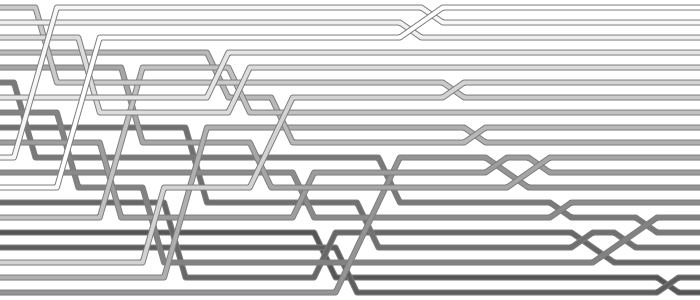
\includegraphics[width=\linewidth]{shell.png}

  \centerline{Algorithme A.}
\end{minipage}\hfill\begin{minipage}{.35\linewidth}
  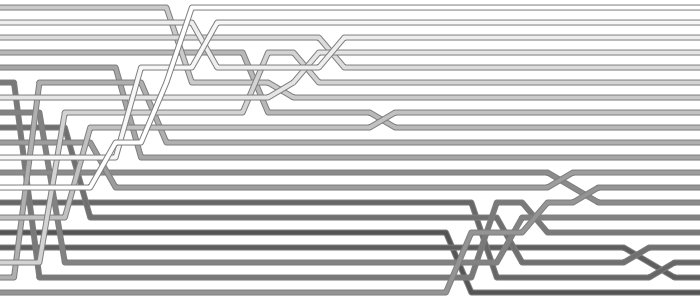
\includegraphics[width=\linewidth]{quick.png}

  \centerline{Algorithme B.}
\end{minipage}\hfill\begin{minipage}{.35\linewidth}
  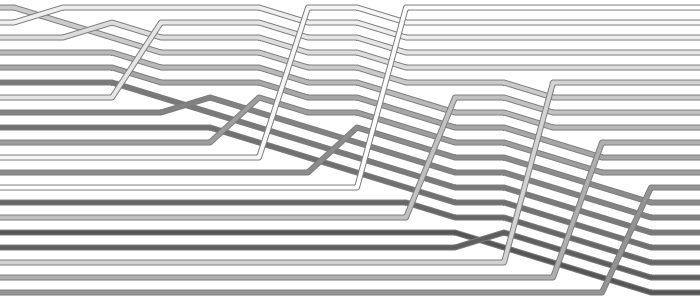
\includegraphics[width=\linewidth]{insertion.png}

  \centerline{Algorithme C.}
\end{minipage}\hfill}~

%%%%%%%%%%%

\noindent\hfill\begin{minipage}{.35\linewidth}
  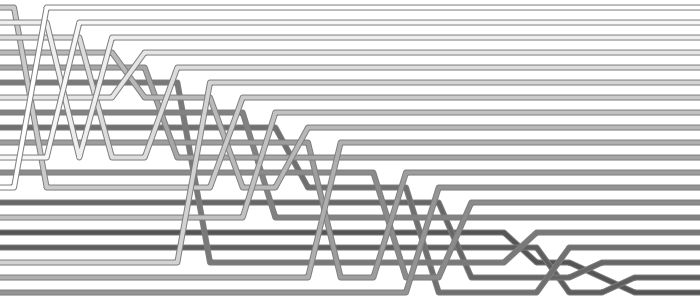
\includegraphics[width=\linewidth]{selection.png}

  \centerline{Algorithme D.}
\end{minipage}\hfill\begin{minipage}{.35\linewidth}
  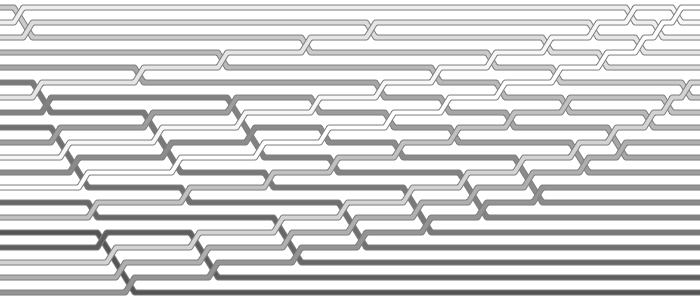
\includegraphics[width=\linewidth]{bubble.png}

  \centerline{Algorithme E.}
\end{minipage}\hfill~

\begin{Reponse}
  \textbf{Tri a bulle:} parcours successifs du tableau en comparant les voisins
  2 à 2. S'ils sont mal triés, on les inverse. Ce comportement a tendance à
  pousser les grosses valeurs vers la fin. On peut reconnaitre ce comportement
  dans l'algorithme B.

  \textbf{Tri par insertion:} invariant: ce qui est avant la frontière est
  trié. A chaque étape, je prend l'élément juste après la frontière, et je le
  met à sa place dans la partie déjà triée. On peut reconnaitre ce comportement
  dans l'algorithme E.

  \textbf{Tri par selection:} a chaque étape, je selectionne le minimum de la
  partie non triée et le pose à la frontière. On reconnait l'algorithme A.

  \textbf{Shell sort:} comme un bubble sort, mais on commence par trier avec un
  écartement supérieur à 1. Au lieu d'inverser des voisins, on inverse des
  cases à distance 3 puis 2 puis on fait un bubble standard, mais sur un
  tableau un peu prétrié. C'est l'algorithme C.

  \textbf{Quick sort:} c'est un algorithme récursif qui trie une partie du
  tableau puis l'autre (les parties ne sont pas forcément de taille
  identique). C'est l'algorithme D.
\end{Reponse}

\end{document}


%%% Local Variables:
%%% coding: utf-8
